
\vspace{1cm}
{\let\clearpage\relax \chapter{Procedimento}} 

Come già descritto, verranno implementati diversi approcci. Per ciascuno di questi, per valutarne le performance predittive, è stata utilizzata la metrica del Mean Absolute Percentage Error (MAPE), dato dalla media aritmentica dei rapporti tra il valore assoluto degli errori di previsione e il valore reale; è inoltre facilmente interpretabile dal punto di vista umano e permette di confrontare i diversi modelli. 



\section{ARIMA}

Per prima cosa è stata analizzata la stazionarietà. È stata osservata una correlazione lineare tra varianza e media a diversi mesi, con R=0.86 e p-value=0.0003, suggerendo l'utilizzo del logaritmo sulla serie. Il test di Augmented Dickey-Fuller, con un p-value di 0.20, conferma inoltre che la serie non è stazionaria in media, e necessita di una differenziazione. 

\begin{figure}[H]
\centering
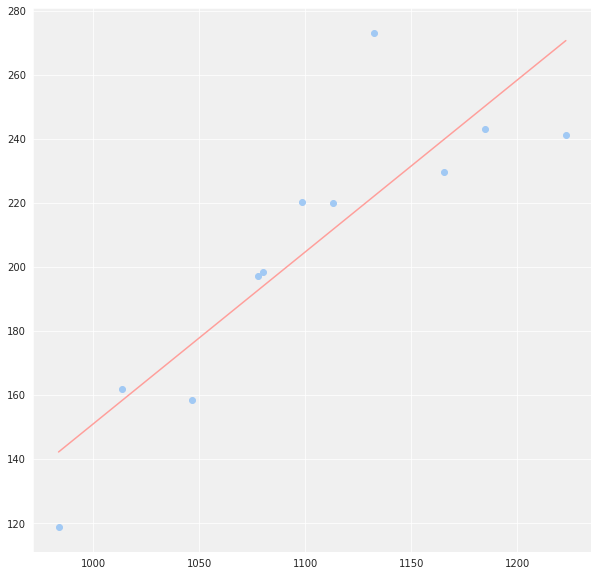
\includegraphics[width=7cm]{Pictures/medie_varianze.png}
\caption{Correlazione lineare tra varianze e medie.}
\end{figure}

Osservando invece i grafici ACF e PACF della serie iniziale, si nota una chiara stagionalità ogni 24 osservazioni (1 giorno), come già notato nella fase iniziale di esplorazione del dataset. 

\begin{figure}[H]
\centering
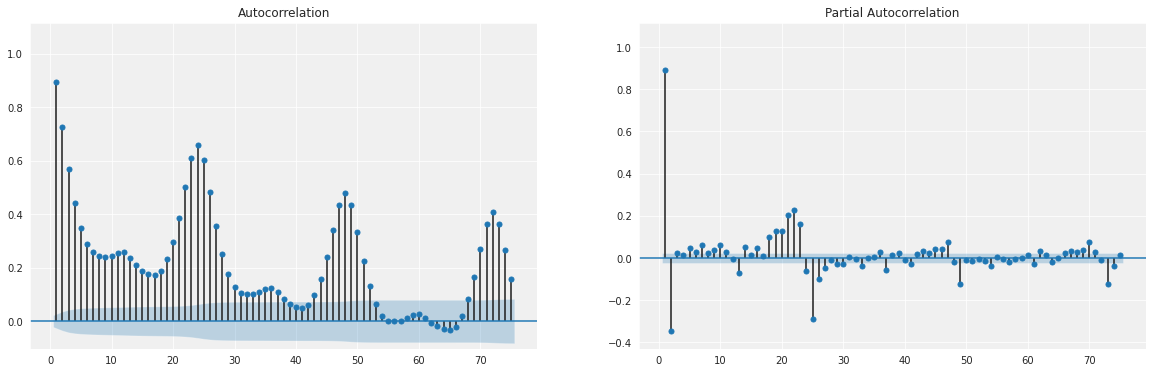
\includegraphics[width=13cm]{Pictures/acf_pacf_1.png}
\caption{ACF e PACF iniziali.}
\end{figure}

Di conseguenza, è stato creato un primo modello, sul logaritmo della serie storica: $ARIMA (0,1,0) (0,1,0) [24]$. Analizzando i suoi residui, si nota come sia necessaria l'aggiunta di un $SMA(1)$, come di solito accade differenziando. 

Viene costruito quindi il modello: $ARIMA (0,1,0) (0,1,1) [24]$. I suoi residui sono migliorati, avendo valori più contenuti nelle bande di confidenza, ma rimane della non stocasticità nei residui stagionali giornalieri. Purtroppo, non è stato individuato un modo per ridurli ulteriormente. Il MAPE sul validation set ha un valore di 11.87\%, mentre un AIC di -19660. 

\begin{figure}[H]
\centering
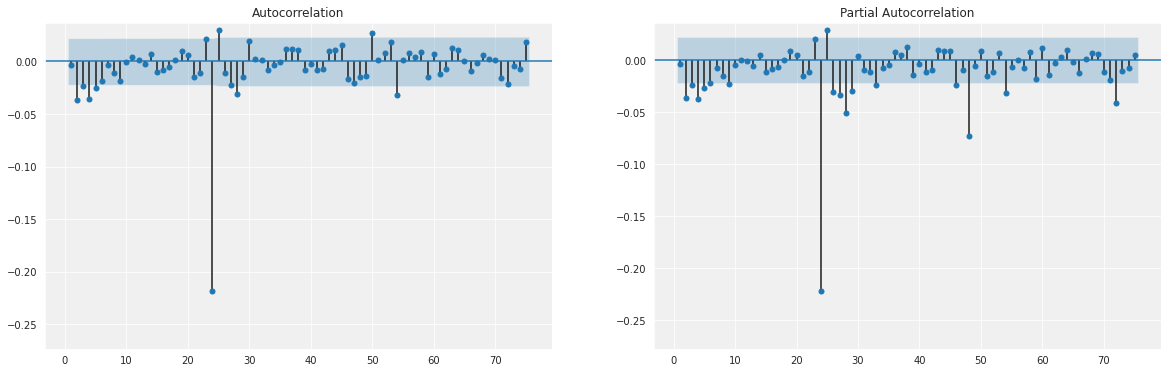
\includegraphics[width=13cm]{Pictures/acf_pacf_2.png}
\caption{ACF e PACF dei residui del modello $ARIMA (0,1,0) (0,1,1) [24]$.}
\end{figure}

Per quanto riguarda i residui a lag inferori, non stagionali, essi non sono direttamente interpretabili a dei valori di $p$ e $q$. Per questo, è stata fatta una grid-search per trovare il modello che modellasse meglio i dati, in termini di AIC e MAPE. I valori risultanti sono $p=2$ e $q=2$, con un MAPE di 11.52\% e un AIC di -20212. 

Si giunge quindi al modello: $ARIMA (2,1,2) (0,1,1) [24]$. Rimane ancora da modellare la stagionalità settimanale, chiaramente visibile nei grafici ACF e PACF a lag più alti. Questa viene modellata utilizzando delle sinusoidi, a periodo 168. 

\begin{figure}[H]
\centering
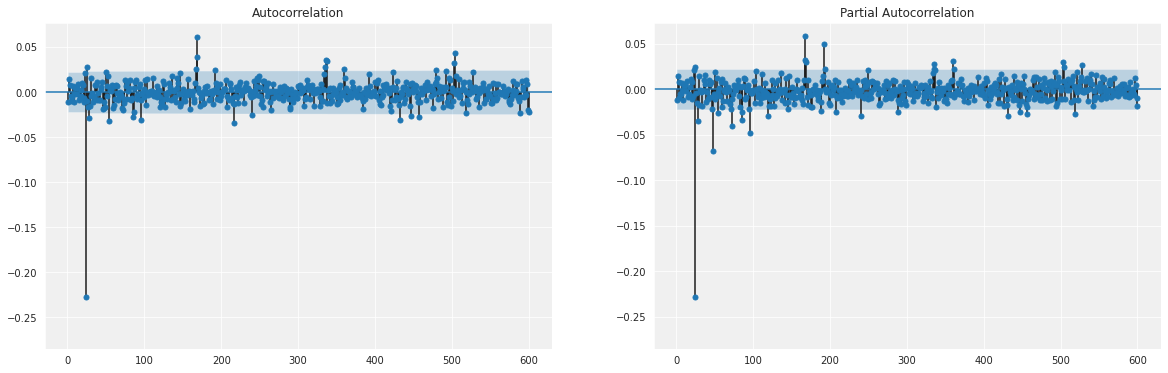
\includegraphics[width=13cm]{Pictures/acf_pacf_3.png}
\caption{ACF e PACF dei residui del modello $ARIMA (2,1,2) (0,1,1) [24]$, questa volta a 600 lag.}
\end{figure}

Dopo un test per verificare quale fosse il numero ottimale di sinusoidi, ovvero 3, è stato creato il modello. Di nuovo, c'è un miglioramento dell'AIC a -20249 e del MAPE sul validation set a 10.94\%. 

Un'ultima versione consiste nell'aggiungere dei regressori dummy per modellare le festività, le quali possono avere dei valori anomali. Dopo un'analisi (manuale) sulla serie storica, si è notato come in poche di essere si verificano eventi fuori dal comune, come il 25 aprile, 2 giugno, 25 dicembre, ecc. Il loro inserimento, in realtà, non comporta miglioramenti in termini di MAPE e di AIC. 

In conclusione, il miglior modello ARIMA presenta un AIC di -20249 e un MAPE di 10.94\%. 

\begin{figure}[H]
\centering
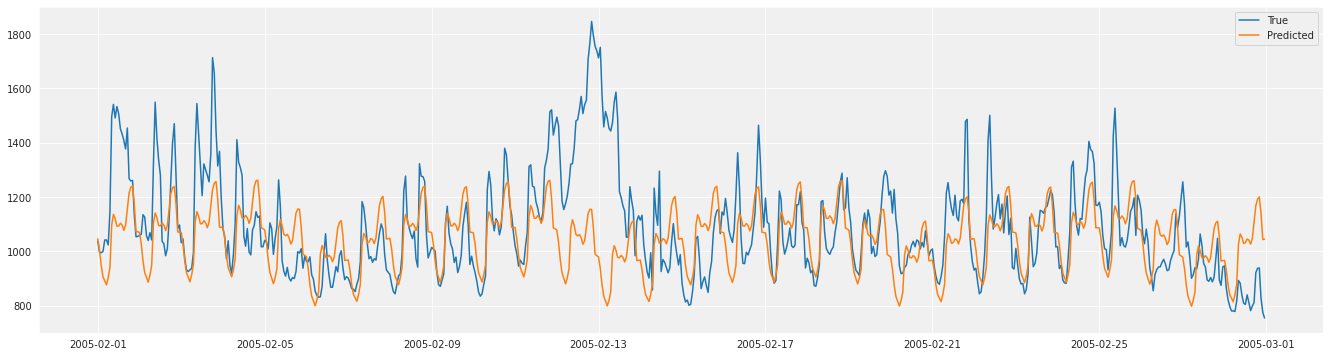
\includegraphics[width=14cm]{Pictures/prediction_arima.png}
\caption{Previsione finale del modello ARIMA.}
\label{plot_arima}
\end{figure}

Dalla figura \ref{plot_arima} si può notare come la stagionalità settimanale sia perfettamente catturata, un po' meno la giornaliera, che è meno stabile nel tempo. Inoltre, i valori anormali del 12-13 febbraio non vengono catturati. 

Infine, individuato il modello più performante, viene verificato che i suoi residui siano generati da un processo white noise, quindi a media nulla, varianza costante e incorrelati con il proprio passato. Mentre i primi due criteri vengono rispettati, l'ultimo non completamente; rimane, infatti, della memoria significativa non modellata. Questo può anche essere causato dal fatto che, trattandosi di dati reali, è difficile ottenere dei residui white noise perfetti.

\vspace{0.5cm}

\begin{figure}[H]
\centering
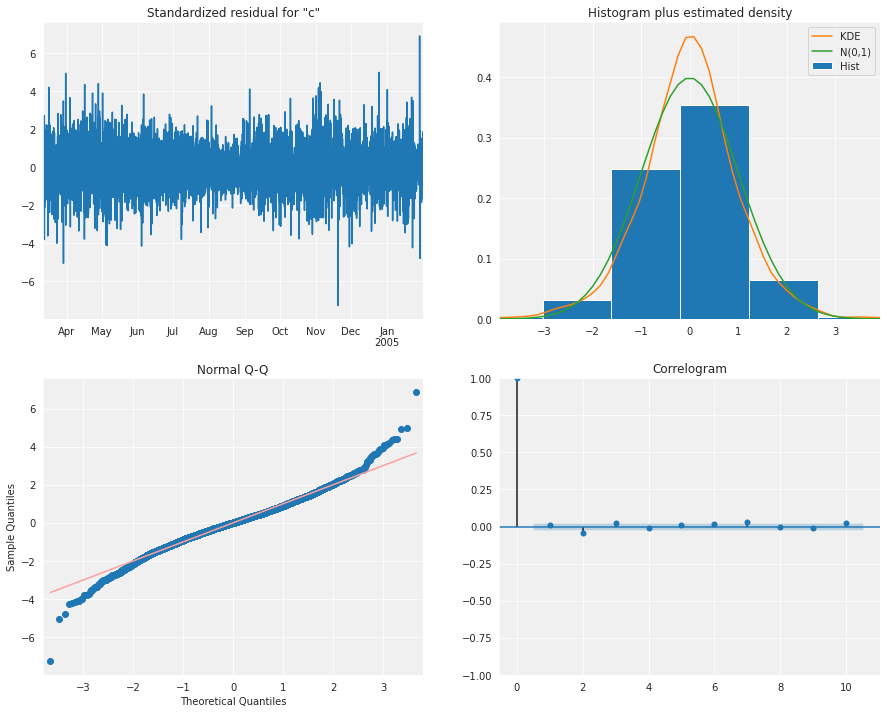
\includegraphics[width=12cm]{Pictures/summary_arima.png}
\caption{Riepilogo sui residui del modello.}
\end{figure}




\section{UCM}

Per questa fase si è deciso di iniziare l’analisi con un modello semplice: conoscendo già i tipi di stagionalità, ne sono state aggiunte una giornaliera dummy e una settimanale sinusoidale, mentre per il level sono stati diversi tipi (random walk, local linear trend, ecc), per determinare il più adatto. 

Individuato il random walk with drift, si è poi passati a verificare se modellare le stagionalità in quel modo fosse effettivamente ottimale. Infatti, si è capito come il modo migliore fosse vederle entrambe scritte come sinusoidi. In particolare, dopo una serie di test, il numero ottimale di sinusoidi è di 5 e 3, rispettivamente per stagionalità stocastica giornaliera e settimanale. È importante notare che, al fine di evitare che l'algoritmo non raggiunga la convergenza, è stata impostata la varianza iniziale del modello ad un valore più consono, cioè la varianza della serie storica di training. 

L'aggiunta della componente di ciclo stocastico non ha portato miglioramenti al modello. Lo stesso vale per l'aggiunta dei regressori esterni dummy sulle festività, così come accadeva anche in ARIMA. 

Quindi, il modello che ottiene le migliori performance, in temini di AIC e MAPE (compromesso tra i due), è quello composto da:
\begin{itemize}
    \item random walk con drift
    \item 6 sinusoidi stocastiche per modellare la stagionalità giornaliera
    \item 2 sinusoidi stocastiche per modellare la stagionalità settimanale
\end{itemize}

Questo modello ottiene un AIC di -19414 e un MAPE di 11.13\%. Si notano, anche graficamente, le minori performance rispetto alla previsione ARIMA. 

\begin{figure}[H]
\centering
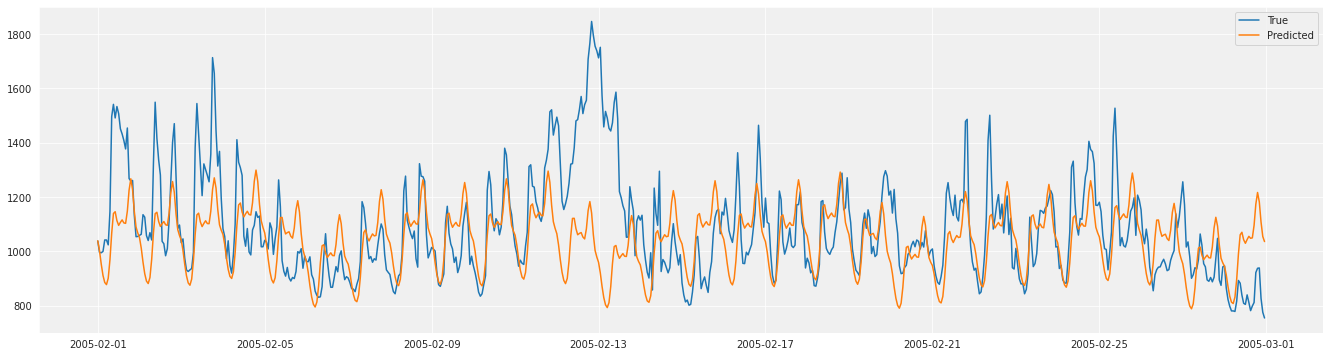
\includegraphics[width=14cm]{Pictures/prediction_ucm.png}
\caption{Previsione finale del modello UCM.}
\end{figure}

I residui del modello finale sono simili a quelli di ARIMA, mantenendo purtroppo ancora più memoria e correlazione. 

\begin{figure}[H]
\centering
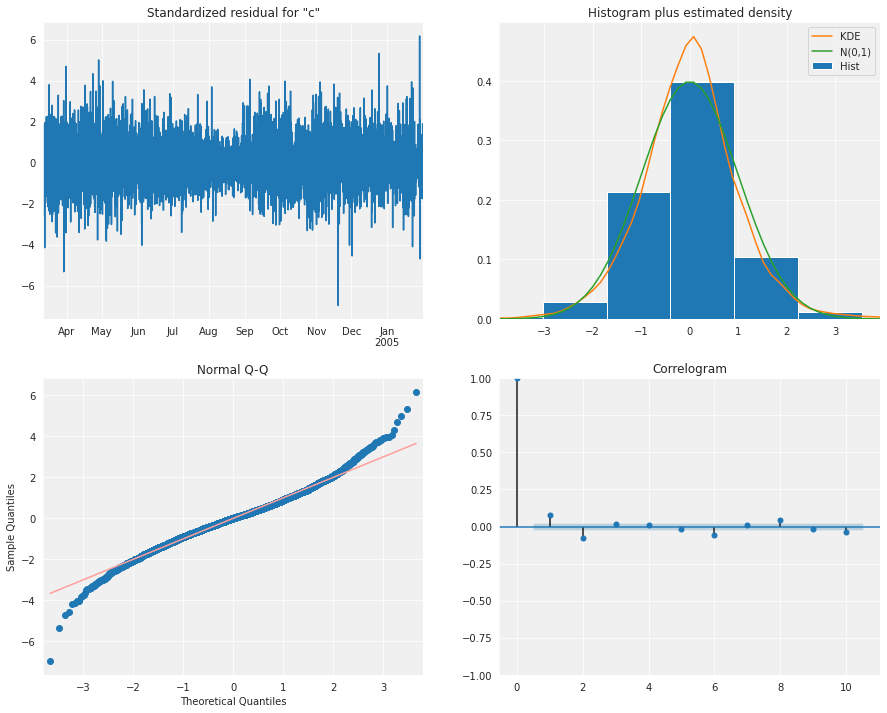
\includegraphics[width=12cm]{Pictures/summary_ucm.png}
\caption{Riepilogo sui residui del modello.}
\end{figure}


\vspace{0.5cm}


\section{Machine Learning}

Sono state implementate diverse tecniche: K-Nearest-Neighbors e Recurrent Neural Networks (Long Short-Term Memory e Gated Recurrent Network)



% -----------------------------------------------------


\subsection{KNN}

L'algoritmo prevede i valori futuri basandosi sui k Nearest Neighbors. Viene utilizzata una metodologia MIMO (multi-input multi-output). 

Per la scelta dei valori degli iperparametri k (numero di osservazioni passate da considerare) e p (quante sottosequenze simili guardare) è stata effettuata una serie di test, andando a prendere quelli che minimizzassero il MAPE sul validation set. I valori testati sono: k in [4, 8, 16, 32, 64] e p in [12, 24, 24*2, 24*4, 24*7, 24*14, 24*21, 24*28]. Si sarebbe potuta effettuare una grid-search più intensa, ma è stato preferito in questo modo al fine di avere una maggiore interpretabilità e velocità di esecuzione. Inoltre, usare la mediana ha fornito risultati leggermente migliori della media. 

I migliori risultano essere $k=8$ e $p = 504$ (tre settimane), ottenendo un MAPE di 10.13\%.

\begin{figure}[H]
\centering
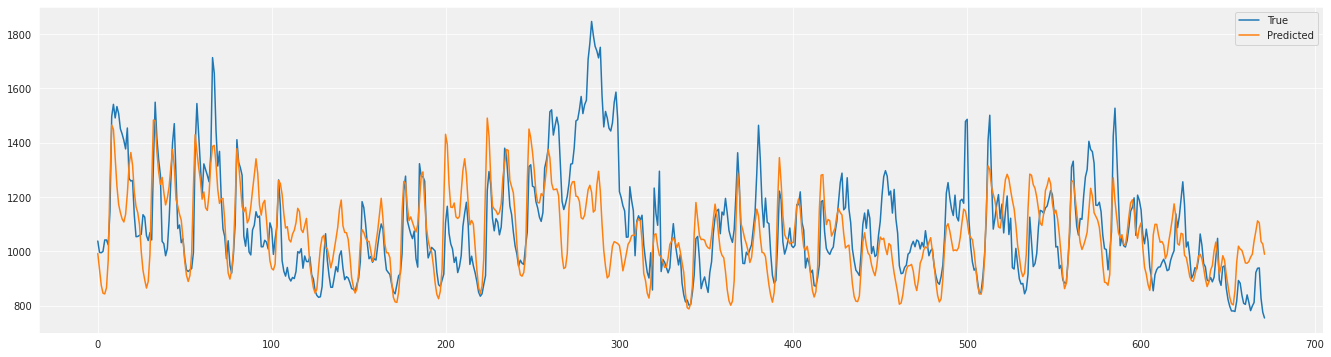
\includegraphics[width=14cm]{Pictures/prediction_knn.png}
\caption{Previsione finale del KNN.}
\end{figure}



% -----------------------------------------------------


\subsection{LSTM}

Per prima cosa, i dati sono stati sottoposti a del preprocessing: oltre ad una normalizzazione tra 0 e 1 (ovviamente rispetto al training set), hanno subito un reshape per essere dati in input alla rete. In particolare, è stata scelta una previsione recursive multi-step, predicendo una settimana alla volta. Questa tecnica fornisce risultati migliori rispetto ad una single-step o ad una multi-step giornaliera. La finestra ottimale sui dati precedenti è di tre settimane.

Sono state effettuate inoltre diverse prove sulla struttura del modello. Il migliore, che cerca di non essere troppo complesso per un trade-off sul tempo di allenamento (i modelli lineari sono estremamente più veloci), è così costruito: 
\begin{itemize}
    \item LSTM di 512 unità, con funzione di attivazione ReLU
    \item Dropout di 0.1
    \item LSTM di 256 unità, con funzione di attivazione ReLU
    \item Dropout di 0.1
    \item Dense di 168 unità (per predizione valori della settimana successiva)
\end{itemize}

Per quanto riguarda il numero di epoche, è stato effettuato un early stopping con patience=3, su 100 epoche, con un batch size di 128 osservazioni.

La previsione avviene settimana per settimana: prendendo in input l'ultimo mese del training set, predice una settimana; aggiorna poi i dati prendendo tre settimane del training set e quella predetta; così via fino ad arrivare ad un mese. Il modello con il MAPE minore risulta essere 10.43\%.

\begin{figure}[H]
\centering
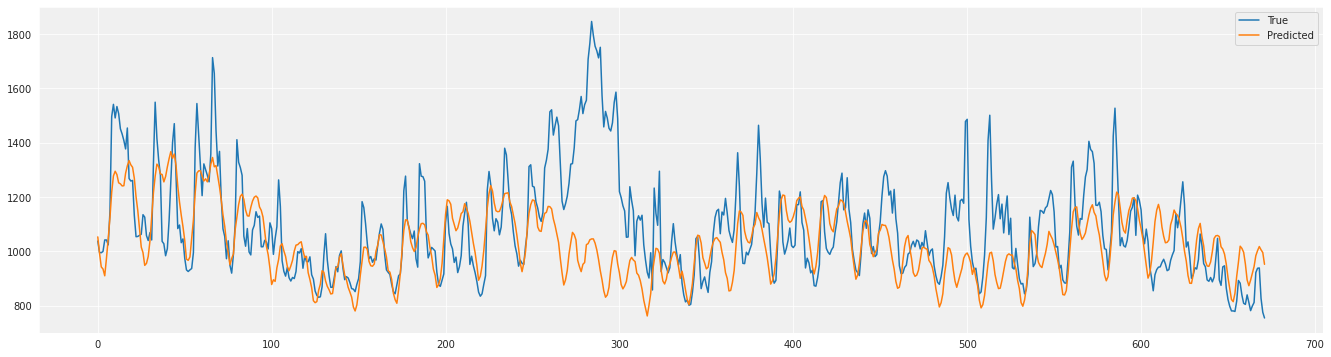
\includegraphics[width=14cm]{Pictures/prediction_lstm.png}
\caption{Previsione finale della RNN con LSTM.}
\end{figure}


% -----------------------------------------------------


\subsection{GRU}

Per le GRU, i dati subiscono lo stesso preprocessing delle LSTM. Anche la struttura della rete viene mantenuta, sostituendo però i layer LSTM con dei layer GRU. Il procedimento è lo stesso in tutto e per tutto, in quanto sembra essere la migliore impostazione anche per questo tipo di RNN. Il modello ottiene un MAPE di 10.93\%

\begin{figure}[H]
\centering
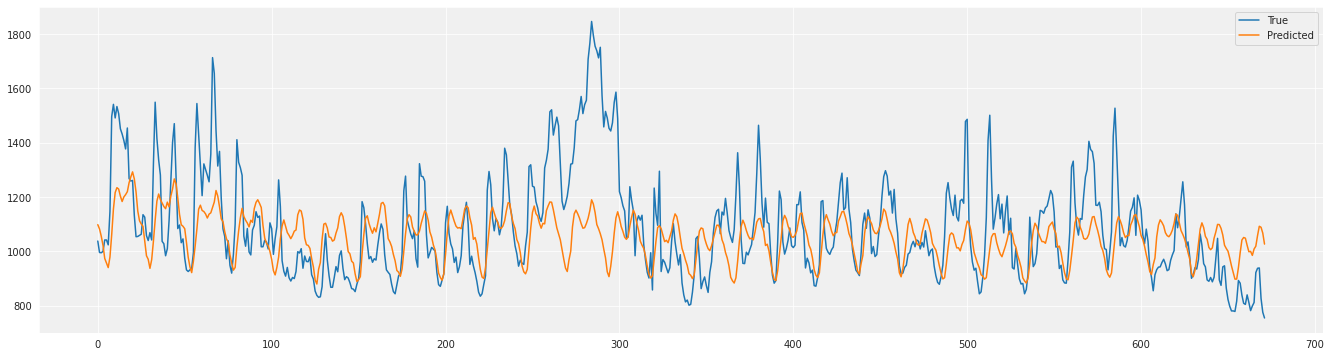
\includegraphics[width=14cm]{Pictures/prediction_gru.png}
\caption{Previsione finale della RNN con GRU.}
\end{figure}






